\section{FANUC setup}
The FANUC robot system required some setup and programming before it could be used as an FDM 3D printing platform. Most of the procedures and settings described in this section can be learned fairly quickly from the lab-style tutorials in \cite{app-programming}. Full documentation is available in the controller manual \cite{lr-handling-tool}.

\subsection{Frames}
The FANUC robot system makes several types of coordinate systems available for defining the robot position and attitude (orientation) in space. These include some pre-defined coordinate systems  that cannot be redefined \cite[sec 3.9]{lr-handling-tool}. The user may define custom coordinate systems attached to the robot or the workspace. These coordinate systems are called "frames" in the teach pendant interface.

For the 3D printing application, a new tool coordinate system and user coordinate system were defined.

\subsubsection{Tool frame}
The new tool frame is attached to the custom end effector with its origin at the tip of the extruder nozzle. The tool frame was defined using the Three Point Method described in \cite[sec~3.9.1]{lr-handling-tool}. The three reference positions (points) used are pictured in Figures~\ref{fig:tool-pt-1} through \ref{fig:tool-pt-3}. An elevated piece of scrap material was used as the tool center reference point to facilitate visual alignment with the nozzle and avoid over-extending the vision camera wire while jogging the robot to the desired approach angles.

\begin{figure}
    \centering
    \begin{subfigure}{.5\textwidth}
        \centering
            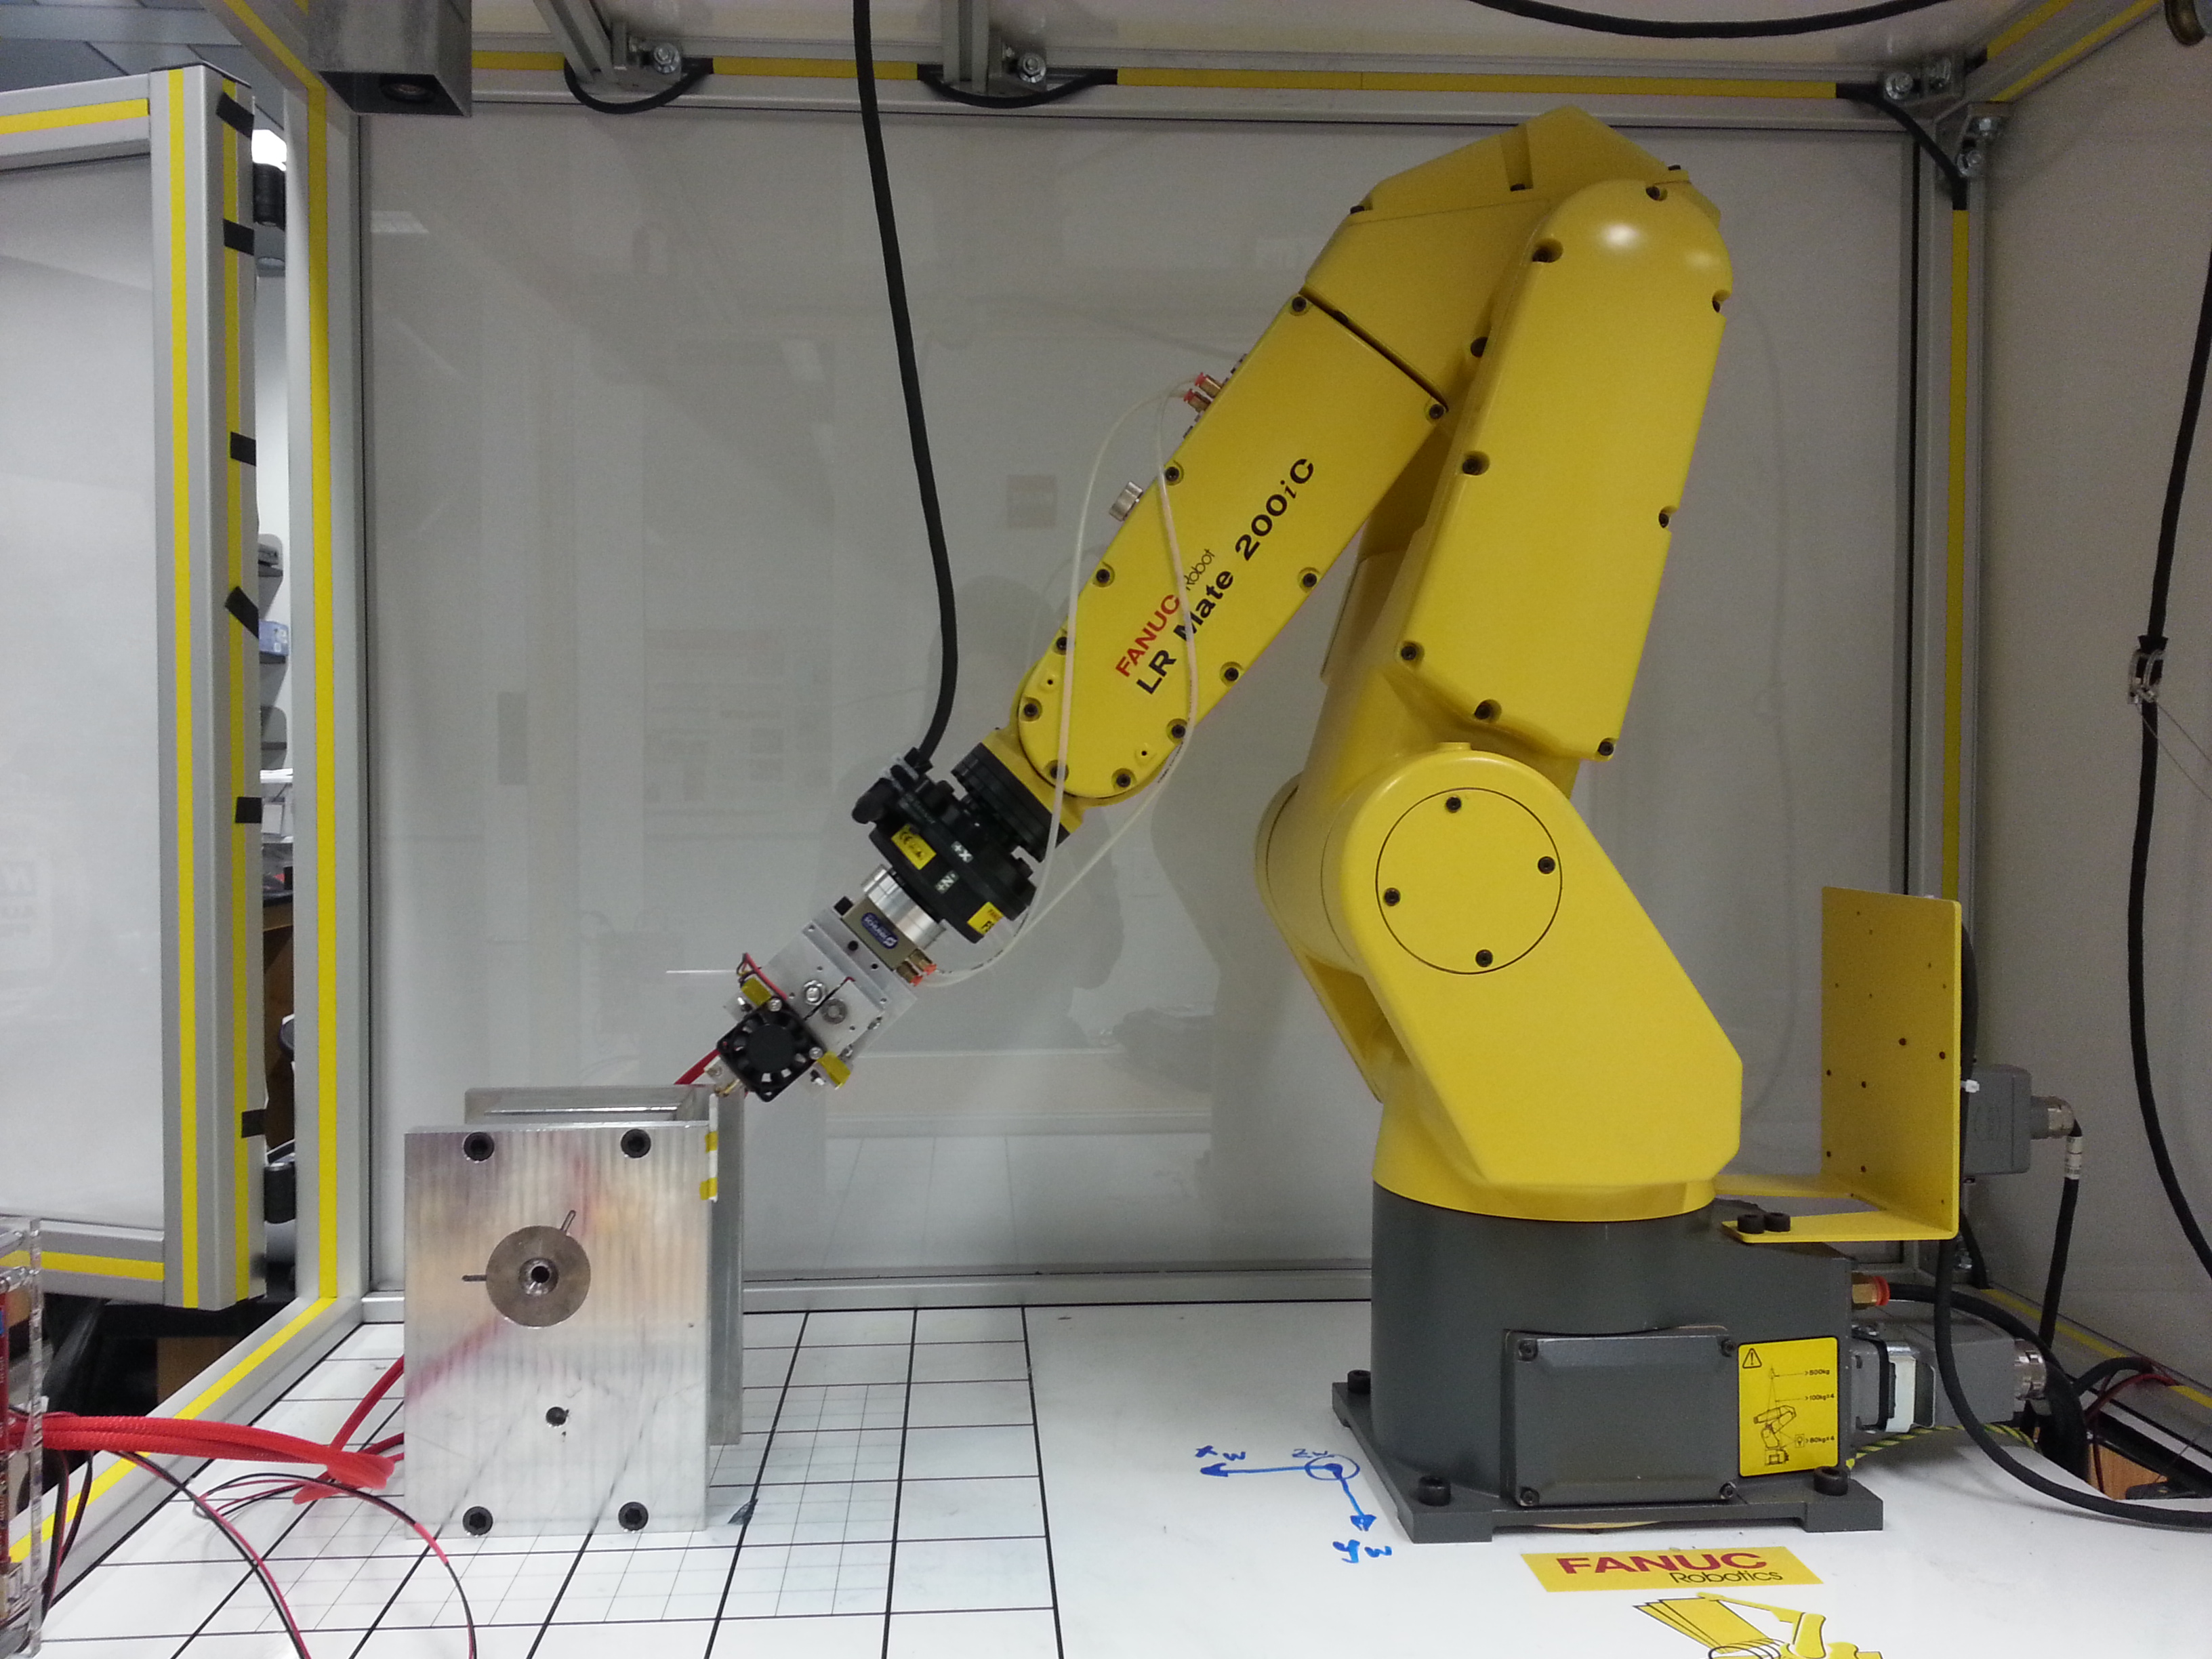
\includegraphics[width=.8\linewidth]{figures/tool-pt-1}
    \end{subfigure}%
    \begin{subfigure}{.5\textwidth}
        \centering
        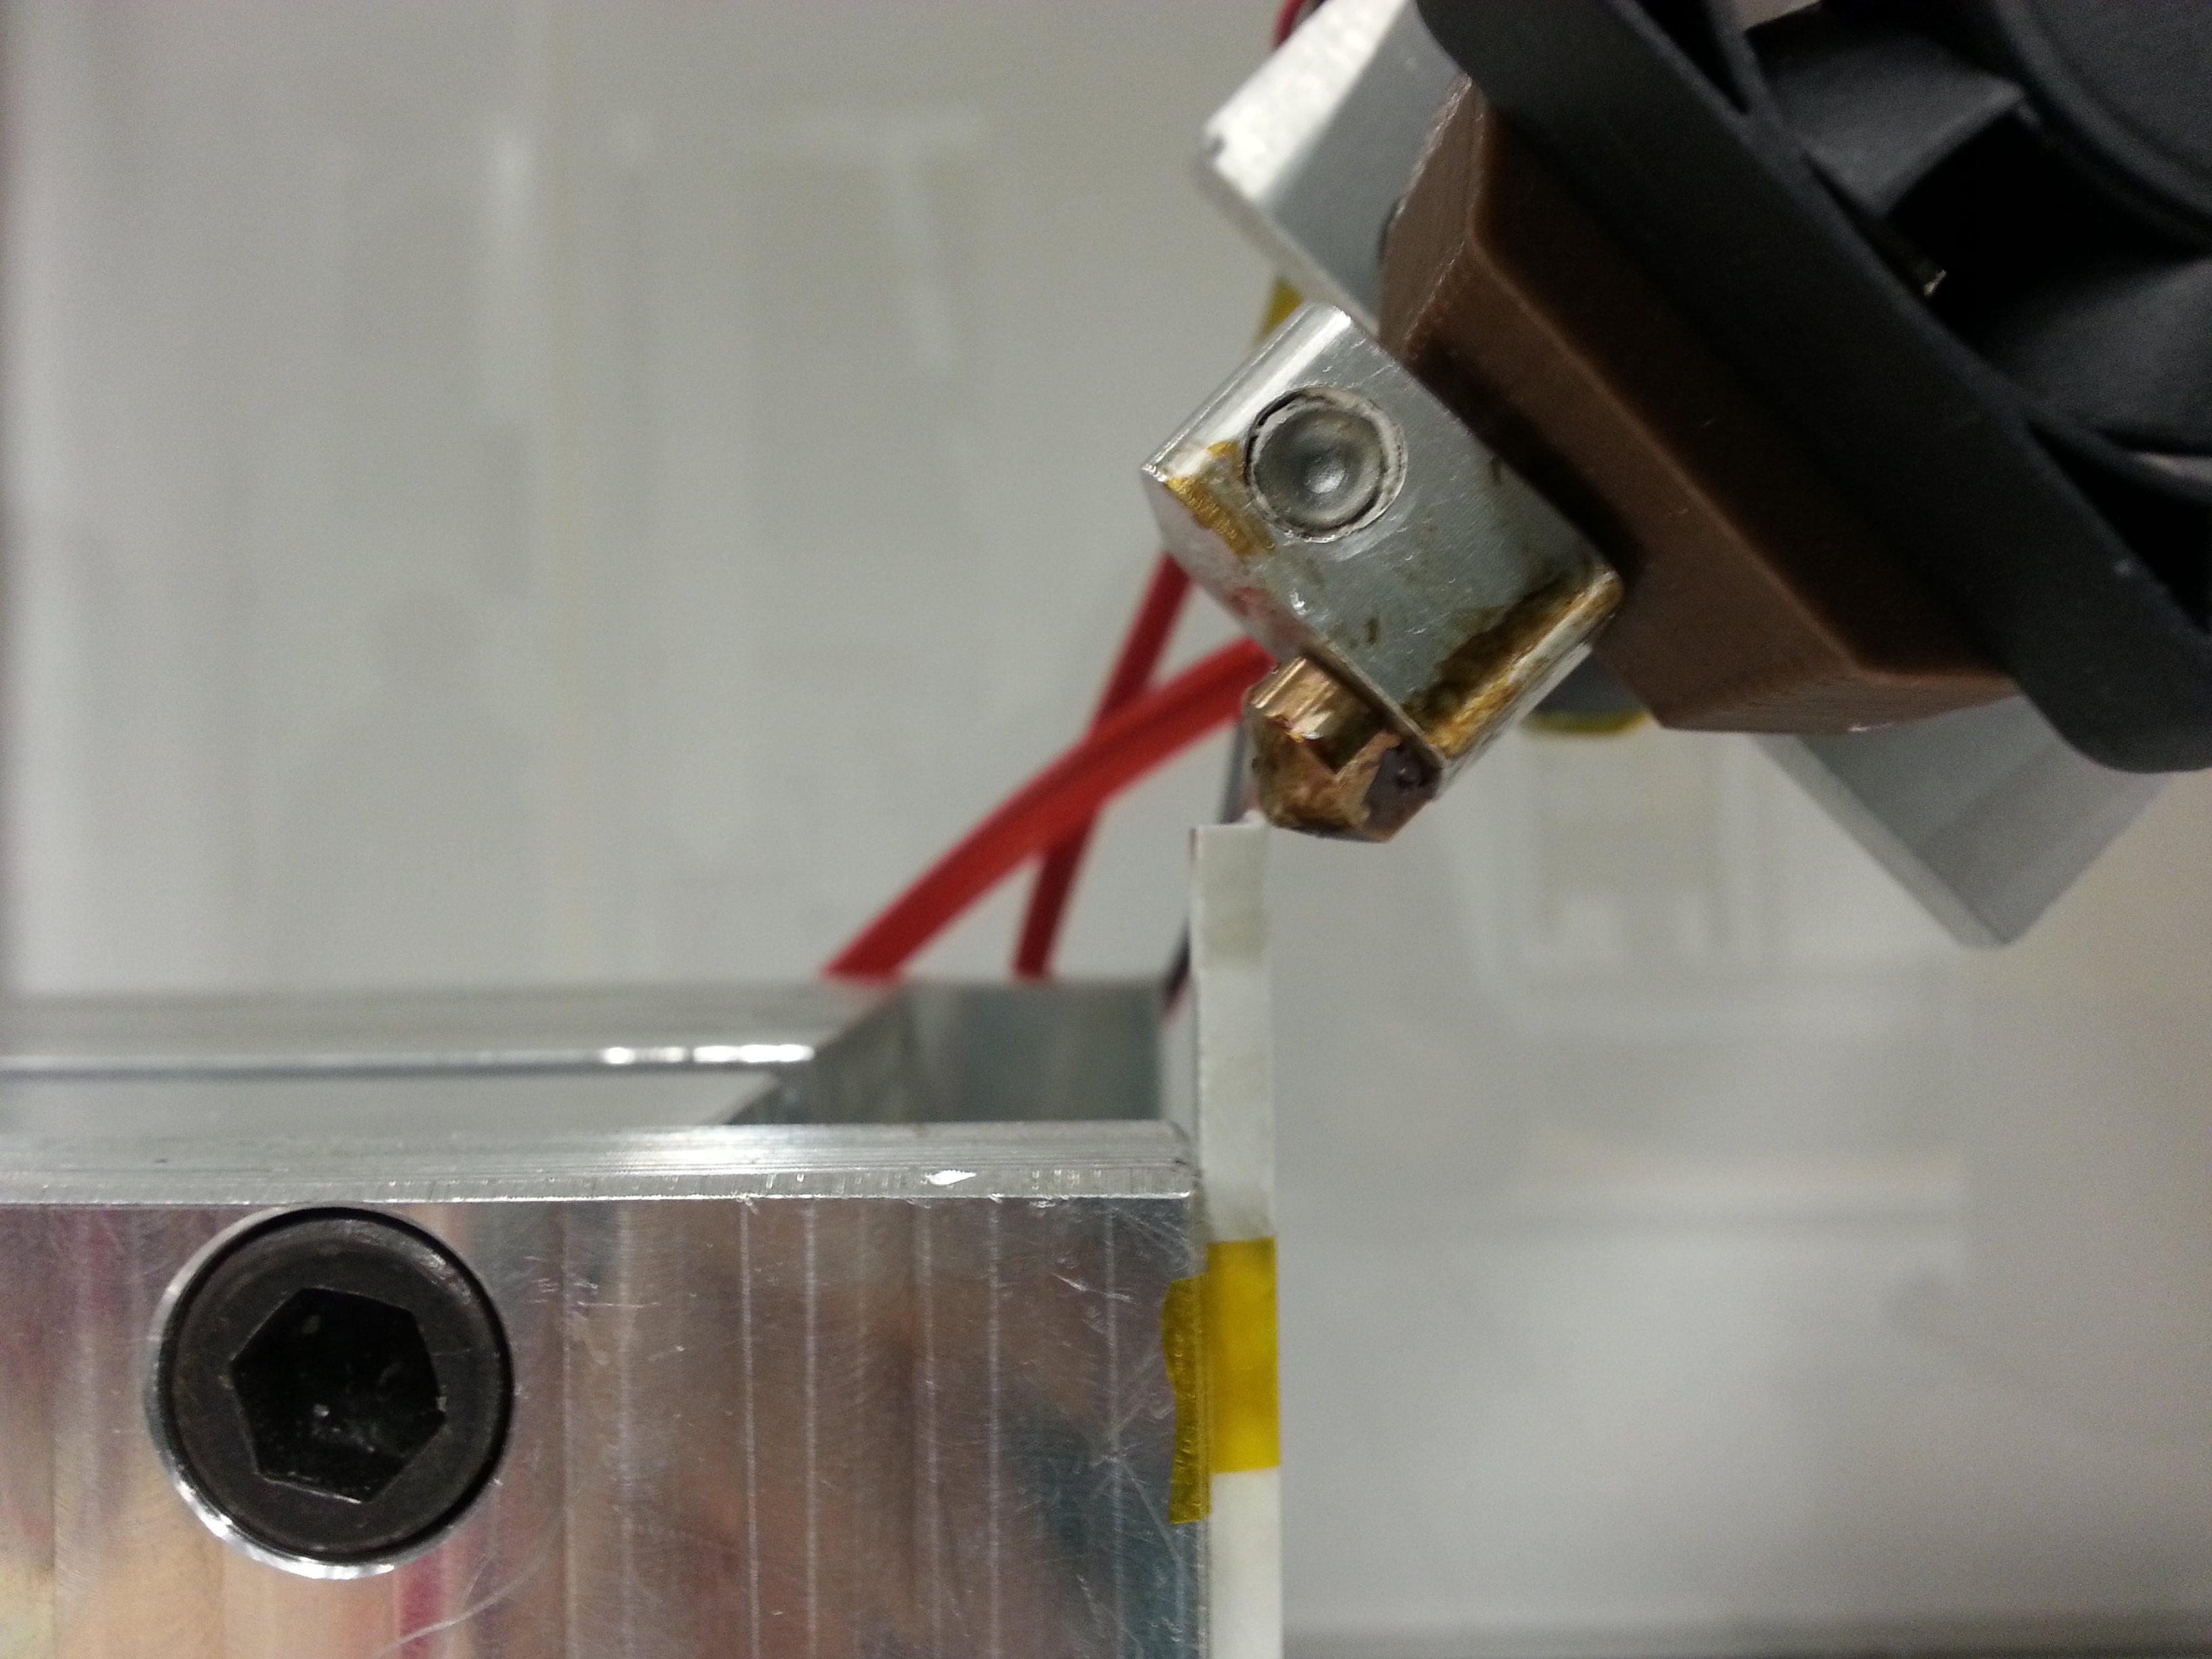
\includegraphics[width=.8\linewidth]{figures/tool-pt-1-close}
    \end{subfigure}
    \caption{Tool Frame reference position 1}
    \label{fig:tool-pt-1}
\end{figure}

\begin{figure}
    \centering
    \begin{subfigure}{.5\textwidth}
        \centering
            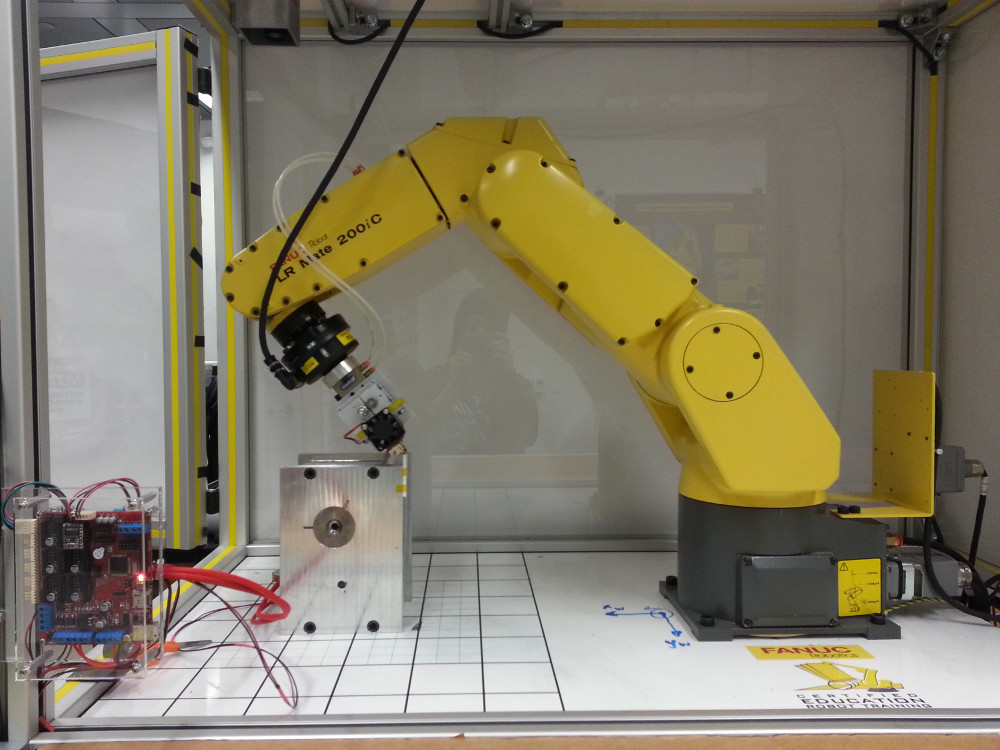
\includegraphics[width=.8\linewidth]{figures/tool-pt-2}
    \end{subfigure}%
    \begin{subfigure}{.5\textwidth}
        \centering
        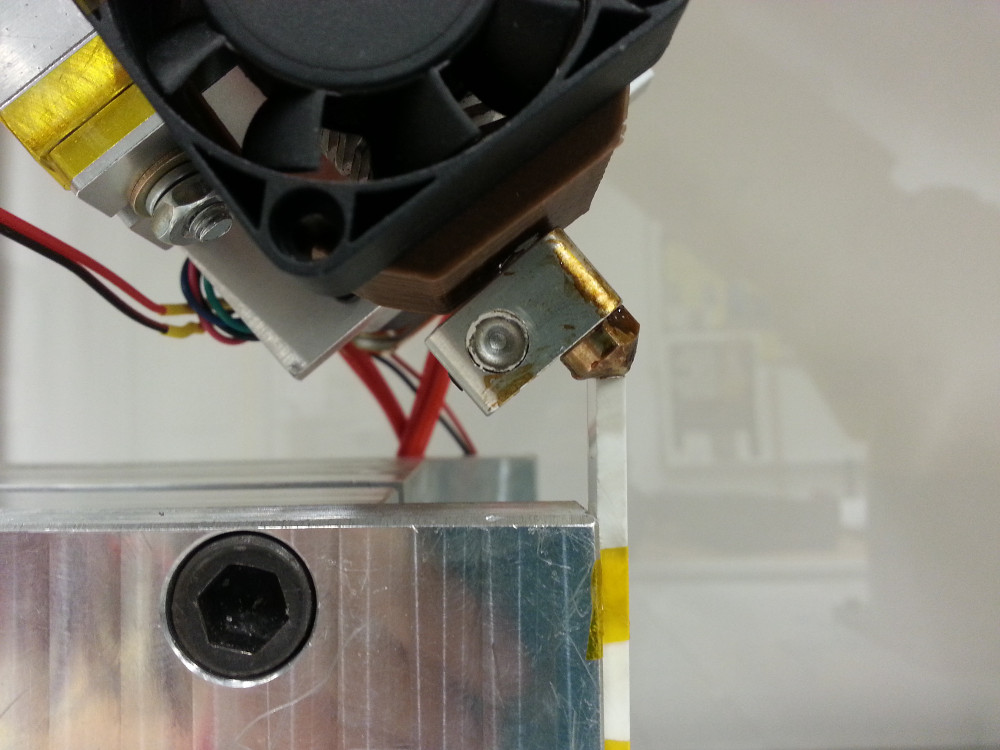
\includegraphics[width=.8\linewidth]{figures/tool-pt-2-close}
    \end{subfigure}
    \caption{Tool Frame reference position 2}
    \label{fig:tool-pt-2}
\end{figure}

\begin{figure}
    \centering
    \begin{subfigure}{.5\textwidth}
        \centering
        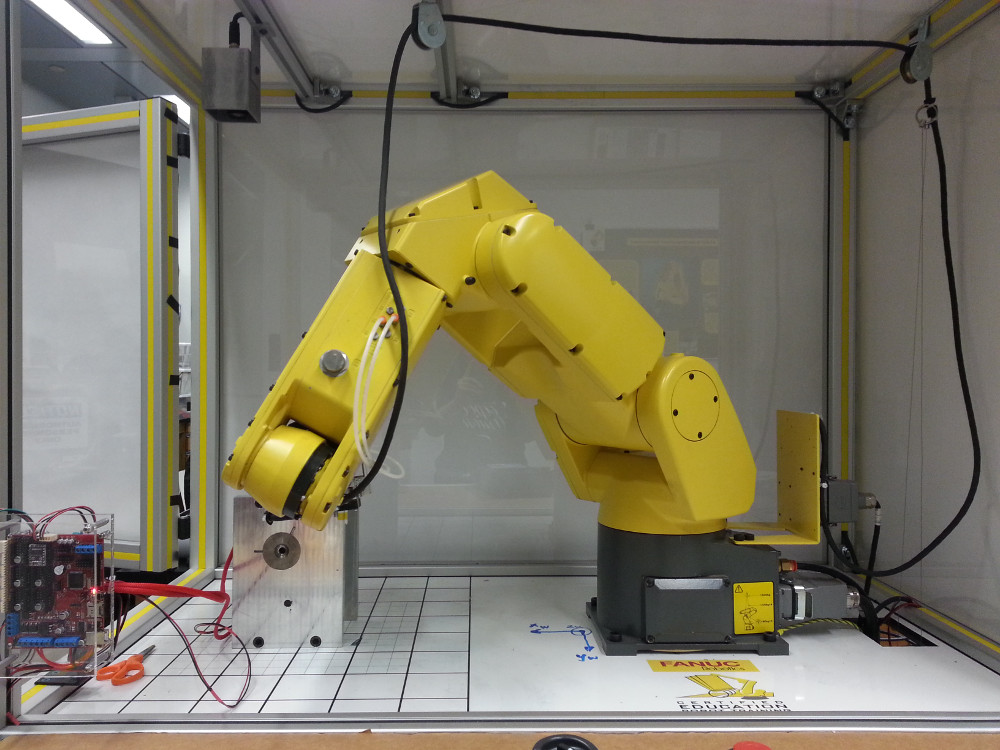
\includegraphics[width=.8\linewidth]{figures/tool-pt-3}
    \end{subfigure}%
    \begin{subfigure}{.5\textwidth}
        \centering
        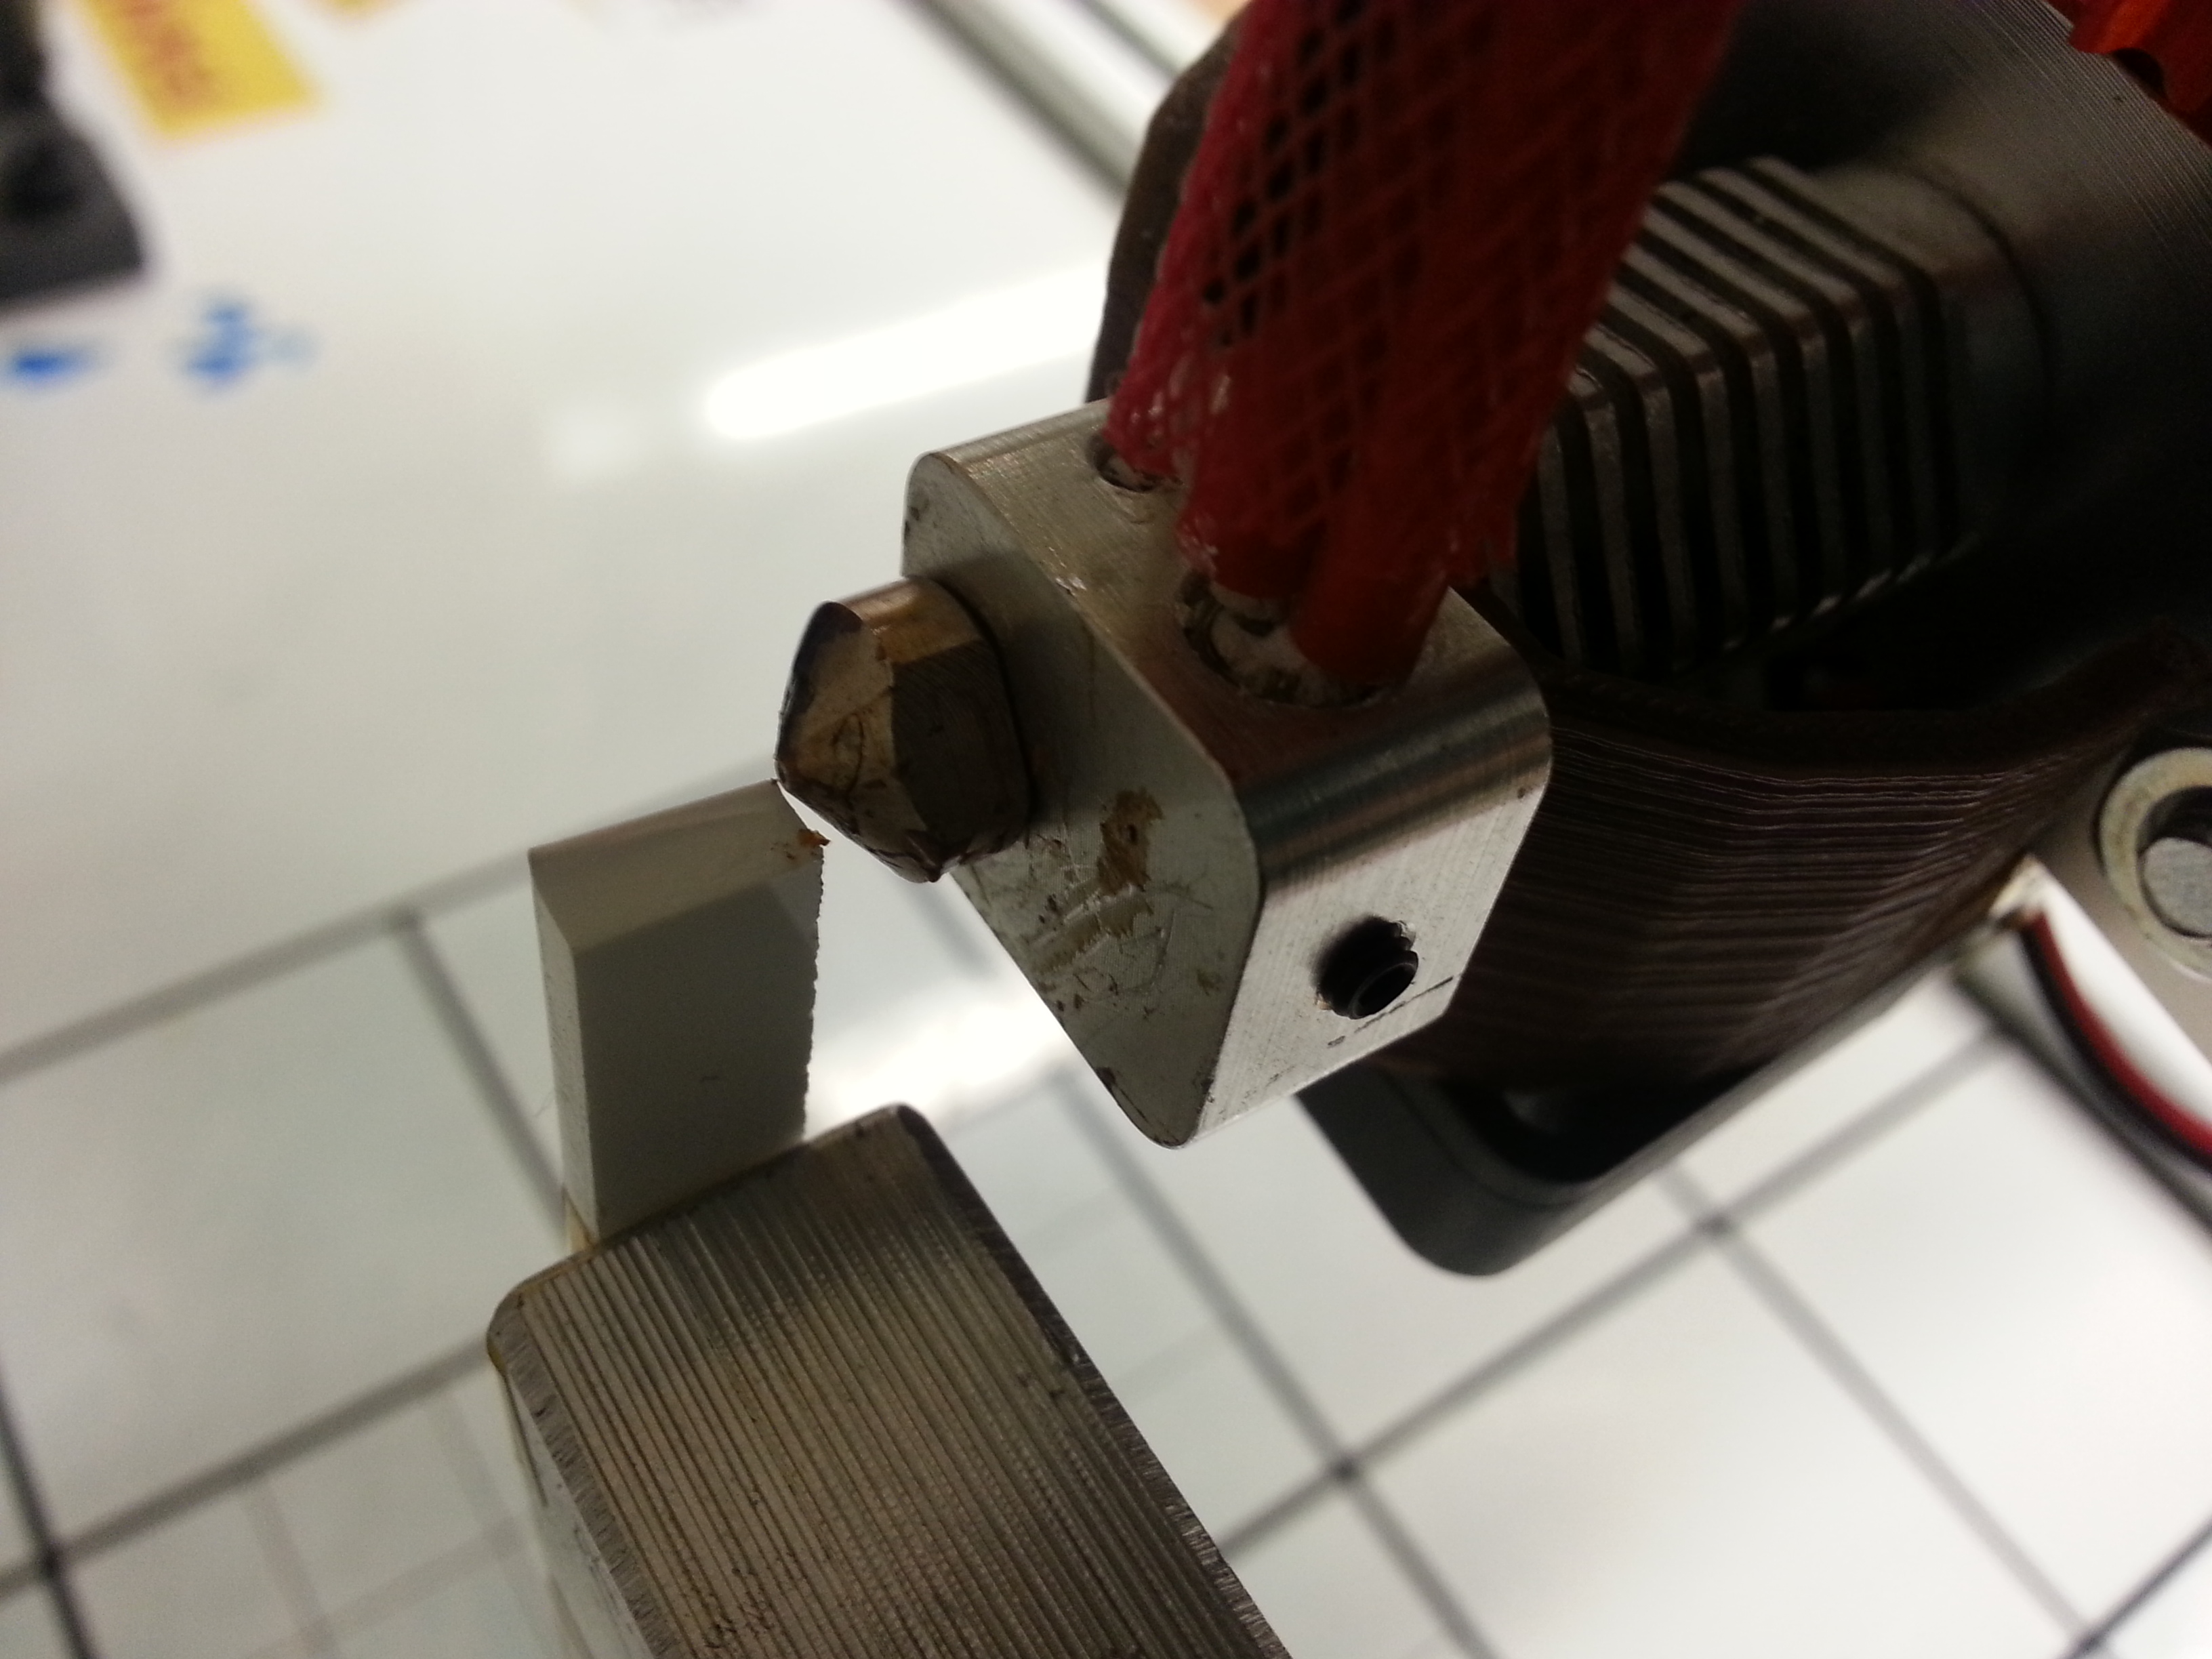
\includegraphics[width=.8\linewidth]{figures/tool-pt-3-close}
    \end{subfigure}
    \caption{Tool Frame reference position 3}
    \label{fig:tool-pt-3}
\end{figure}

\subsubsection{User frame}
The new user frame is attached to the robot workspace and is used as the coordinate system for 3D printing. The user frame was defined using the Direct List Method described in \cite[sec~3.9.2]{lr-handling-tool}. Assuming the dry-erase board surface would be used for printing, and that it lies in the x-y plane of the robot World frame\footnote{Both assumptions may become problematic if the board surface is not sufficiently flat or parallel to the x-y plane of the World frame. A new print surface and User frame may be required. Existing FDM (closed- and open-source) solutions may give clues.}, the z-coordinate of the new user frame was determined by touching the nozzle tip to the board and recording the z-coordinate of the robot in the World frame. A sheet of paper was placed under the nozzle tip to indicate a touch, shown in Figure~\ref{fig:nozzle-touch}. 

\begin{figure}
    \centering
    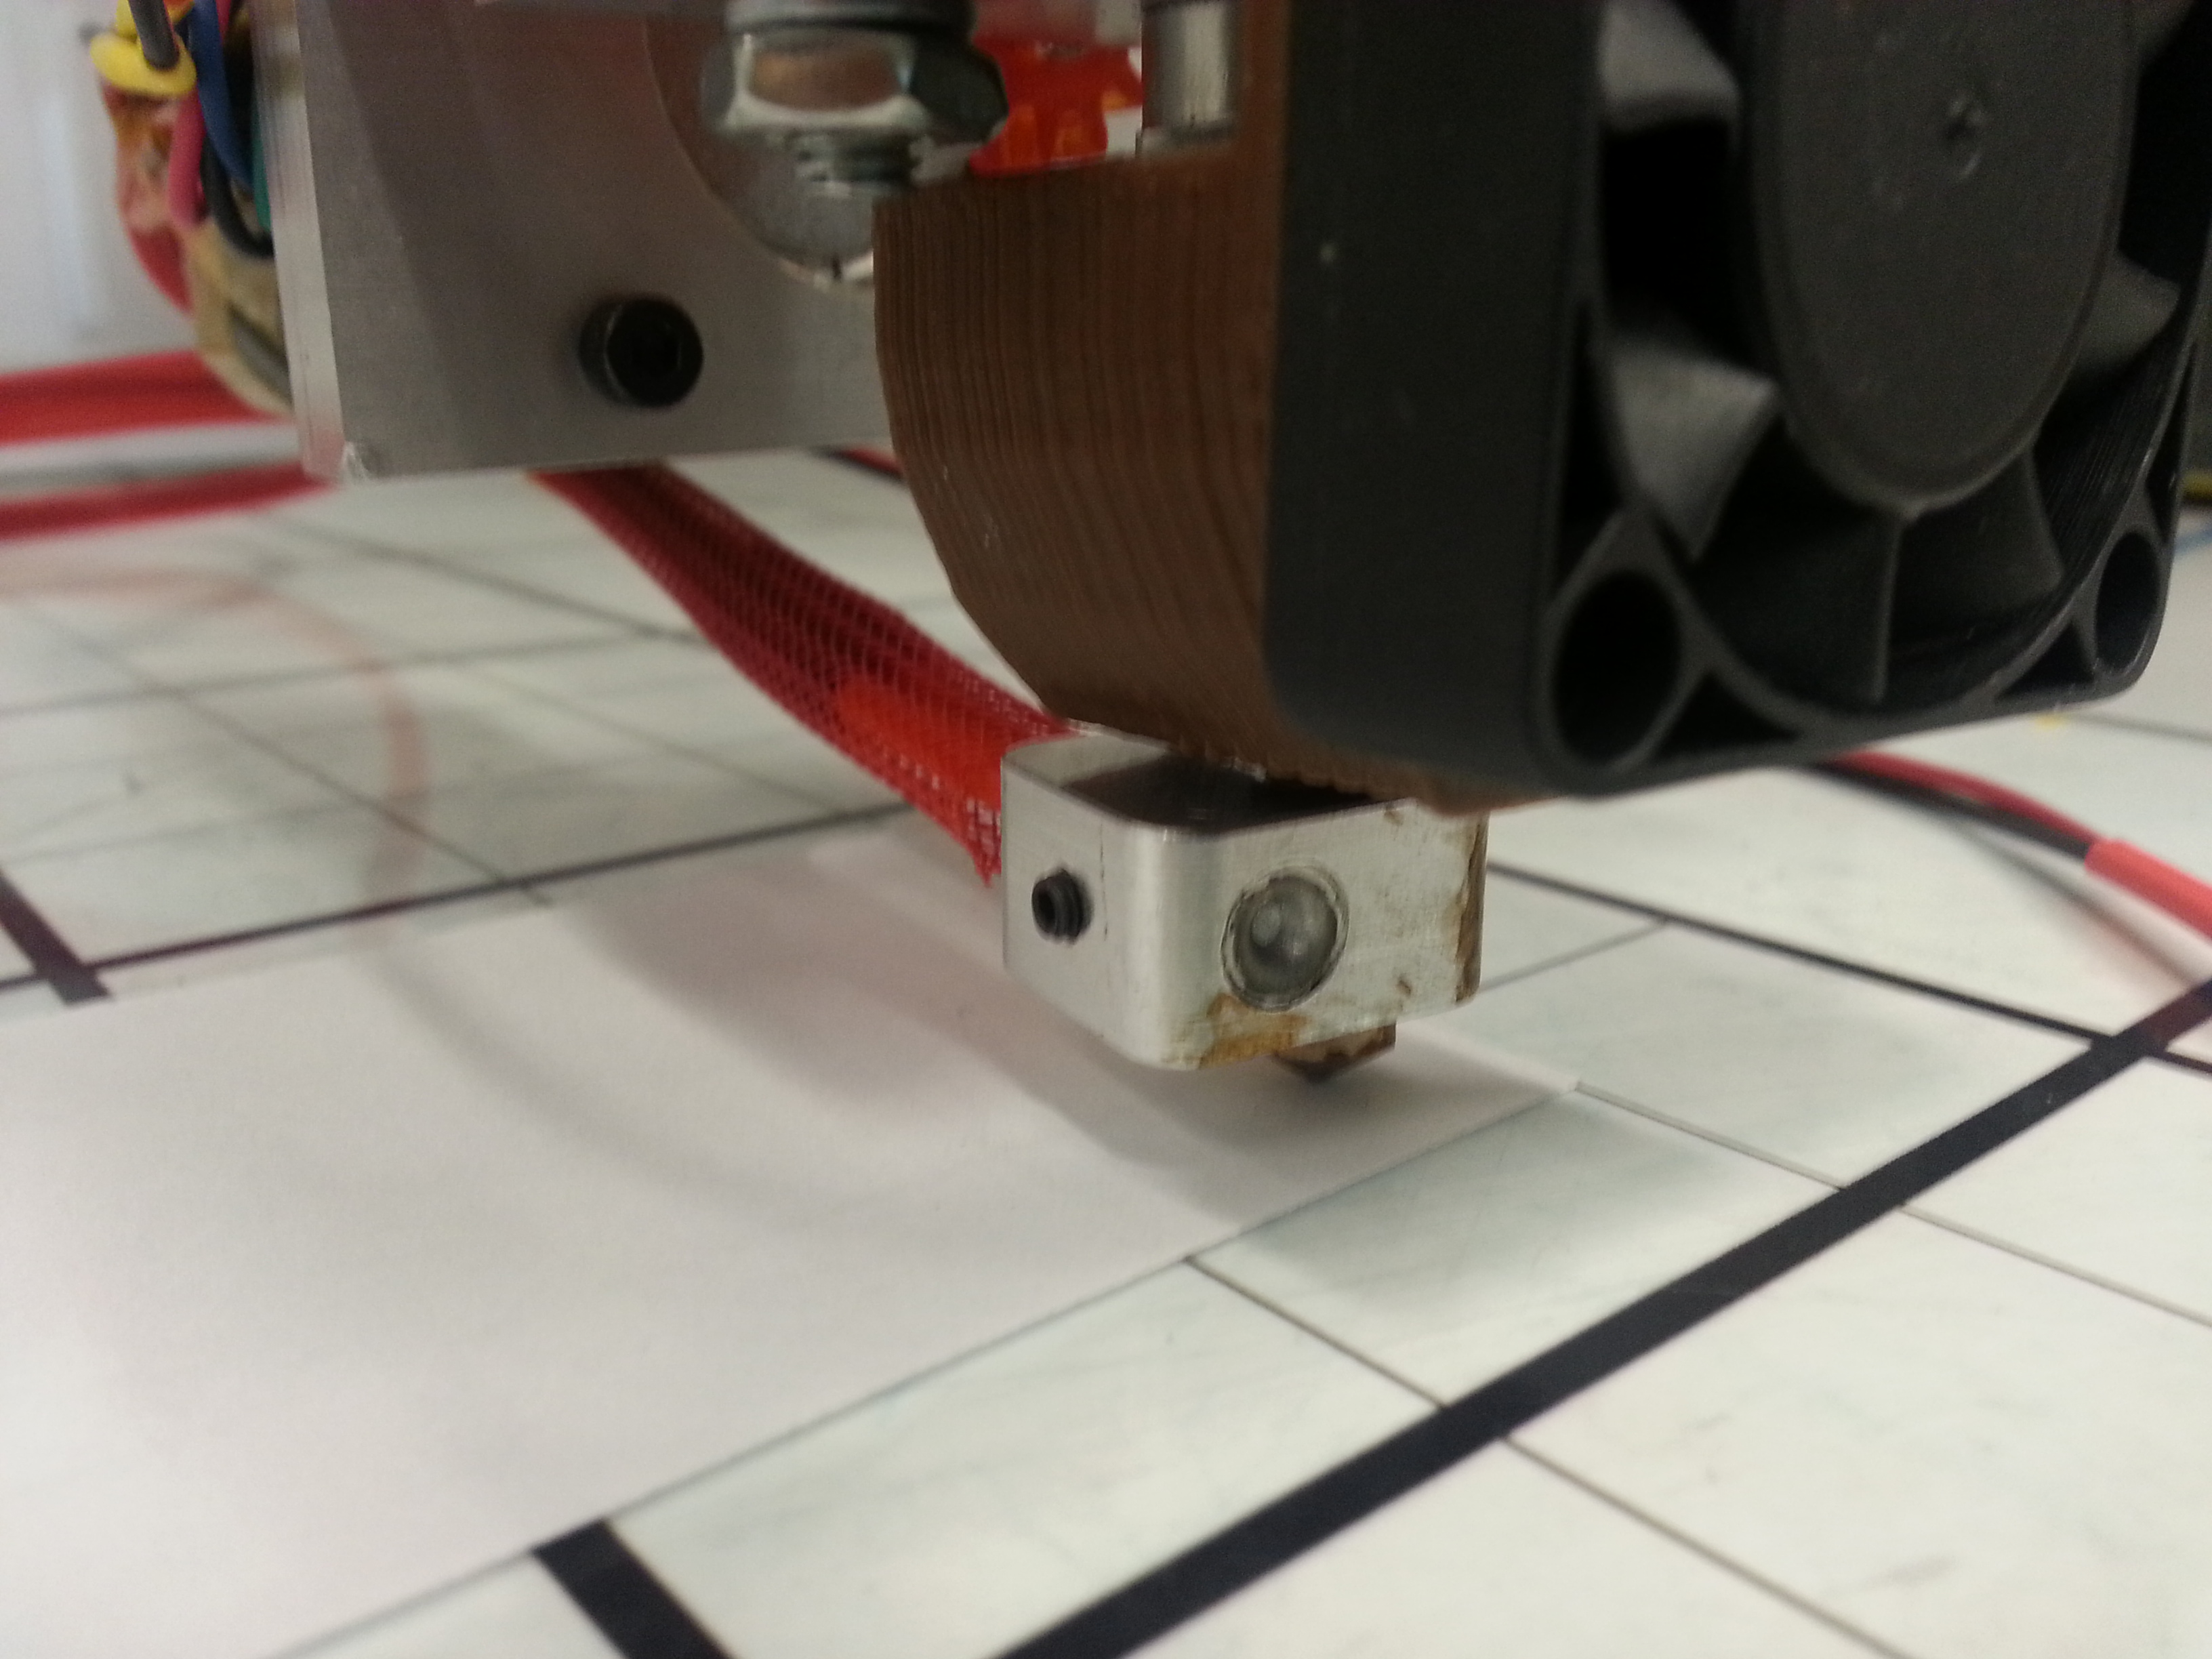
\includegraphics[width=.8\linewidth]{figures/nozzle-paper}
    \caption{User frame nozzle touch test}
    \label{fig:nozzle-touch}
\end{figure}

\subsection{Programming}
The FANUC R30iA Mate controller can be programmed from the attached Teach Pendant, pictured in Figure~\ref{teach-pendant}.

\begin{figure}
    \centering
    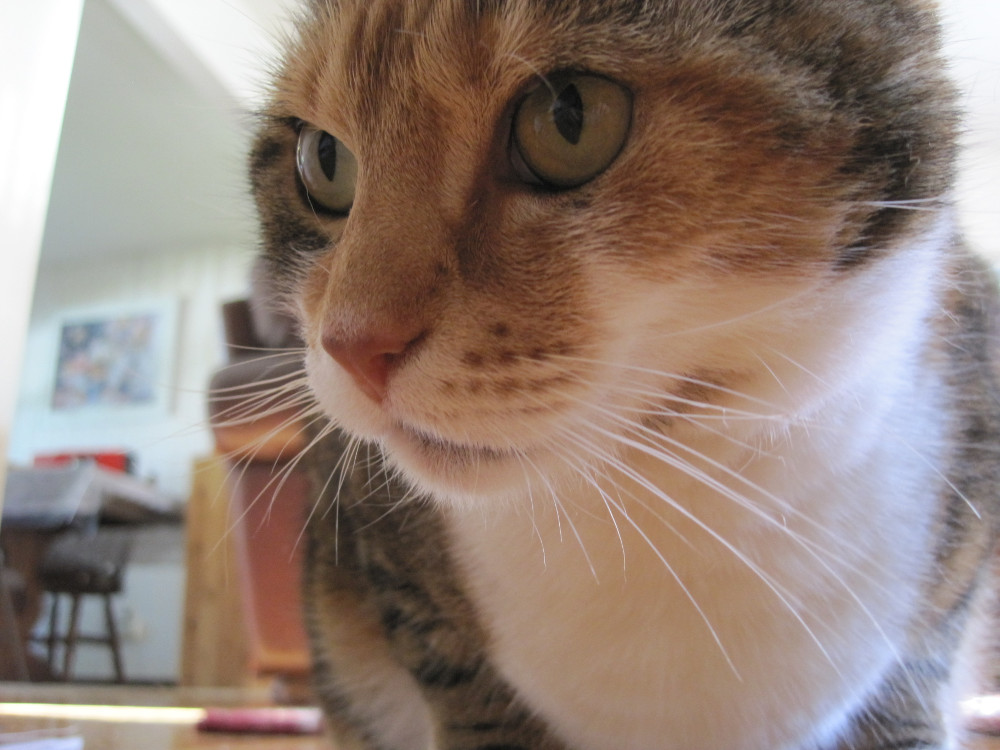
\includegraphics[width=.8\linewidth]{figures/temp-cat}
    \caption{FANUC R30iA Mate Teach Pendant}
    \label{fig:teach-pendant}
\end{figure}


\begin{verbatim}
 1:  UFRAME_NUM=4                            // set user frame
 2:  UTOOL_NUM=4                             // set user tool frame
 3:  R[4:layer num]=0                        // reset layer counter
 4:  PR[12:layer frame RW]=                  // set layer RW (read+write) frame 
  :  PR[11:layer frame R]                       position register   
 5:  R[5:contour num]=0                      // reset contour counter
 6:  PR[13,2:contour offset]=0               // reset contour offset
 7:  R[7:contour incr dir]=(-1)              // reset contour increment direction
 8:  TOOL_OFFSET_CONDITION                   // set tool offset condition to  
  :  PR[13:contour offset]                      contour offset
 9:  LBL[2]                                  // label 2: layer loop
10:  UFRAME[4]=PR[12:layer frame RW]         // set user frame to incremented 
  :                                             layer frame
11:  LBL[1]                                  // label 1: contour loop
12:J  P[1] 100% FINE Tool_Offset             // joint move to point 1
13:J  P[2] 100% FINE Tool_Offset
14:C  P[3] Tool_Offset                       // circular interpolation 
  :   P[4] 250mm/sec FINE Tool_Offset           thru pt 3 to pt 4
15:C  P[5] Tool_Offset
  :   P[6] 250mm/sec FINE Tool_Offset
16:C  P[7] Tool_Offset
  :   P[8] 250mm/sec FINE Tool_Offset
17:J  P[9] 100% FINE Tool_Offset
18:  PR[13,2:contour offset]=(               // increment contour offset 
  :  PR[13,2:contour offset]+                   position register
  :  R[6:contour incremnt]*
  :  R[7:contour incr dir]))
19:J  P[9] 100% FINE Tool_Offset
20:C  P[8] Tool_Offset
  :   P[7] 250mm/sec FINE Tool_Offset
21:C  P[6] Tool_Offset
  :   P[5] 250mm/sec FINE Tool_Offset
22:C  P[4] Tool_Offset
  :   P[3] 250mm/sec FINE Tool_Offset
23:J  P[2] 100% FINE Tool_Offset
24:J  P[1] 100% FINE Tool_Offset
25:  R[5:contour num]=R[5:contour num]+1     // increment contour counter
26:  IF R[5:contour num]>=31,JMP LBL[3]      // don't increment after last 
                                                contour pair
27:  PR[13,2:contour offset]=(
  :  PR[13,2:contour offset]+
  :  R[6:contour incremnt]*
  :  R[7:contour incr dir]))
28:  JMP LBL[1]
29:  LBL[3]
30:  R[4:layer num]=R[4:layer num]+1         // increment layer counter
31:  PR[12,3:layer frame RW]=                // increment layer frame 
  :  PR[12,3:layer frame RW]+.1                 position register
32:  R[7:contour incr dir]=                  // invert contour increment
  :  R[7:contour incr dir]*(-1)                 direction
33:  IF R[4:layer num]<31,JMP LBL[2]
[END]
\end{verbatim}


\subsection{Motion commands}

\subsubsection{Position registers}
\subsubsection{Data registers}
\subsection{Toolpath point generation}

\subsection{Speed output signal}
\begin{verbatim}
1:	R[3:machine speed]=$SCR_GRP[1].$MCH_SPD
2:	AO[1]=R[3:machine speed]
[END]
\end{verbatim}

